\documentclass[11pt]{article}

\usepackage[T1]{fontenc}
\usepackage{mathtools,amsthm,amssymb}
\usepackage{lmodern}
\usepackage{microtype}
\usepackage[margin=1.05in]{geometry}
\usepackage{enumitem}
\usepackage{needspace}
\usepackage{xcolor}
\usepackage{tikz}
\usetikzlibrary{arrows.meta}
\pdftrailerid{}
\pdfsuppressptexinfo=15
\usepackage{hyperref}
\hypersetup{colorlinks=true,linkcolor=black,citecolor=black,
  urlcolor=blue!45!black,pdftitle={The second Kahn--Kalai conjecture},
  pdfauthor={Rewritten for readability from the OpenAI manuscript of the same title}}

\newtheorem{theorem}{Theorem}[section]
\newtheorem{lemma}[theorem]{Lemma}
\newtheorem{fact}{Fact}
\renewcommand{\thefact}{\Alph{fact}}
\numberwithin{equation}{section}

\newcommand{\PP}{\mathbb P}
\newcommand{\EE}{\mathbb E}
\newcommand{\pc}{p_{\mathrm c}}
\newcommand{\pE}{p_{\mathrm E}}
\newcommand{\ind}{\mathbf 1}
\newcommand{\TT}{\mathcal T}
\newcommand{\UU}{\mathcal U}
\newcommand{\ch}{\operatorname{Ch}}
\newcommand{\ee}{\mathrm e}

\newcommand{\unverified}[1]{\par\smallskip\noindent\fbox{\parbox{0.95\linewidth}{\textbf{Unverified step.} #1}}\par\smallskip}
\newcommand{\step}[2]{\medskip\noindent\textbf{Step #1 (#2).}\ }

\title{The second Kahn--Kalai conjecture}
\author{Rewritten for readability from the OpenAI manuscript of the same title}
\date{}

\begin{document}
\maketitle
\begin{abstract}
For every finite simple graph $H$ with $h\ge1$ edges and at most $n$
vertices, the threshold for $G(n,p)$ to contain a copy of $H$ is at most
$C\,\pE(n,H)(1+\log_2 h)$ with a universal constant $C$, where
$\pE(n,H)$ is the least density at which every subgraph of $H$ has
expected copy count at least one half. This is the second Kahn--Kalai
conjecture. The proof given here is self-contained and uses only
elementary probability.
\end{abstract}

\section{The result and an overview of the proof}\label{sec:introduction}

\subsection{Statement}

All graphs are finite and simple. A \emph{copy} of $F$ in $G$ is a
subgraph of $G$ isomorphic to $F$, where a subgraph consists of a set of
vertices of $G$ and a set of edges of $G$ among them. Copies need not be
induced. Write $N(G,F)$ for the number of copies of $F$ in $G$. Let
$G(n,p)$ be the random graph on $[n]=\{1,\ldots,n\}$ in which each of
the $\binom n2$ possible edges is present independently with
probability $p$. For a graph $H$ with at least one edge and at most $n$
vertices, define
\begin{align*}
 \pc(n,H)
 &=\inf\{p\in[0,1]:\PP(N(G(n,p),H)>0)\ge\tfrac12\},\\
 \pE(n,H)
 &=\inf\{p\in[0,1]:\EE N(G(n,p),F)\ge\tfrac12
                 \text{ for every subgraph }F\subseteq H\}.
\end{align*}
The first is the \emph{containment threshold}, the second the
\emph{graph expectation threshold}. Four elementary facts will be used.
\begin{enumerate}[label=(\alph*),leftmargin=2.2em,itemsep=2pt]
 \item Each copy of $F$ in $K_n$ is present in $G(n,p)$ with
 probability $p^{e(F)}$, so
 \begin{equation}\label{eq:firstmoment}
  \EE N(G(n,p),F)=N(K_n,F)\,p^{e(F)}.
 \end{equation}
 \item \emph{Both infima are attained.} By \eqref{eq:firstmoment} each
 constraint in $\pE$ defines a closed subset of $[0,1]$. It contains
 $p=1$ because $N(K_n,F)\ge1$ when $F$ has at most $n$ vertices. There
 are finitely many $F$. Likewise $\PP(N(G(n,p),H)>0)$ is a polynomial
 in $p$ with value $1$ at $p=1$.
 \item \emph{$\pE(n,H)>0$.} For $F$ a single edge the constraint is
 $\binom n2 p\ge\frac12$.
 \item \emph{$\pE(n,H)\le\pc(n,H)$.} If $H$ appears with probability
 at least $\frac12$, so does every $F\subseteq H$, and
 $\EE N\ge\PP(N>0)$.
\end{enumerate}

\begin{theorem}\label{thm:main}
For every $n\ge2$ and every finite simple graph $H$ with $h=e(H)\ge1$
edges and at most $n$ vertices,
\begin{equation}\label{eq:stronger}
 \pc(n,H)\le
 \min\{1,\;2048\ee^{50}\pE(n,H)(1+\log_2 h)\}.
\end{equation}
In particular,
\[
 \pc(n,H)\le6144\ee^{50}\pE(n,H)\log_2 n.
\]
\end{theorem}

Here $\ee$ is the base of the natural logarithm. The constants are
universal, and $H$ may vary with $n$. Kahn and Kalai use expected count
one instead of one half. By \eqref{eq:firstmoment} the constraint of a
subgraph with $x\ge1$ edges then changes by the factor $2^{1/x}\le2$,
so the expectation threshold changes by a factor between $1$ and $2$
and the conjecture is the same.

\subsection{Proof at a glance}\label{sec:glance}

A probability law on subsets $A$ of a finite set $X$ is
\emph{$a$-spread} if $\PP(J\subseteq A)\le a^{|J|}$ for every nonempty
$J\subseteq X$. The proof has three layers.

\begin{center}
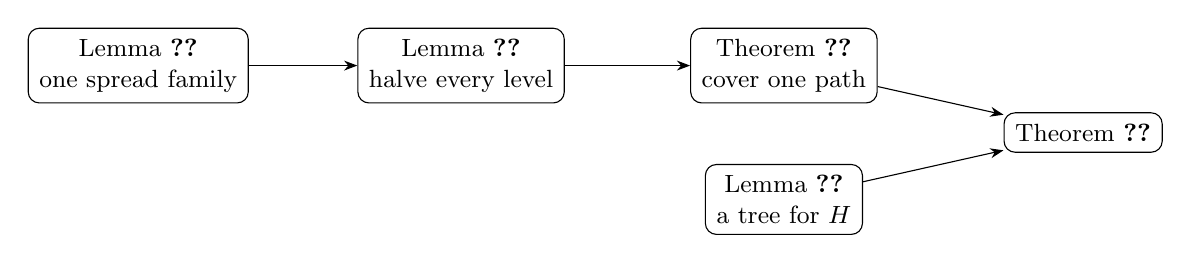
\begin{tikzpicture}[>=Stealth, every node/.style={font=\small},
  box/.style={draw, rounded corners, align=center, inner sep=4pt}]
\node[box] (loc) at (0,0) {Lemma~\ref{lem:local}\\ one spread family};
\node[box] (red) at (4.1,0) {Lemma~\ref{lem:reduction}\\ halve every level};
\node[box] (tree) at (8.2,0) {Theorem~\ref{thm:tree}\\ cover one path};
\node[box] (hier) at (8.2,-1.7) {Lemma~\ref{lem:hierarchy}\\ a tree for $H$};
\node[box] (main) at (12,-0.85) {Theorem~\ref{thm:main}};
\draw[->] (loc)--(red);
\draw[->] (red)--(tree);
\draw[->] (tree)--(main);
\draw[->] (hier)--(main);
\end{tikzpicture}
\end{center}

\noindent\textbf{Layer 3: graphs give a tree (Lemma~\ref{lem:hierarchy}).}
Put $q=\pE(n,H)$. One builds a chain of edge sets
$\varnothing=H_0\subset H_1\subset\cdots\subset H_k=H$ and a rooted
tree. A node at depth $i$ is a copy of $H_i$ on $[n]$, together with the
copies of $H_1,\dots,H_{i-1}$ through which it was reached. Its children
are all copies of $H_{i+1}$ containing it, chosen uniformly. The arc to
a child is labelled by the set of added edges. The chain is chosen by a
maximisation, and this has two consequences. First, the first-moment
constraints at density $q$ force $|H_{i-1}|<|H_i|/17$, so label sizes
grow by a factor of at least $16$ per level. Second, maximality makes
every child law $128q$-spread. Labels along a root-to-leaf path are
disjoint and their union is a copy of $H$.

\smallskip\noindent\textbf{Layer 2: covering a path of a tree
(Theorem~\ref{thm:tree}, Lemma~\ref{lem:reduction}).}
Consider any tree with labels disjoint along paths, $\sigma$-spread
child laws and label sizes growing by a factor of $16$. Then a random
set of density $16\ee^{50}\sigma(1+\log_2\ell_k)$ contains all labels of
some root-to-leaf path with probability at least $\frac23$. Here
$\ell_k$ bounds the largest label size. The proof iterates a
\emph{reduction}. One random set $W$ of density $\rho=4\ee^{50}\sigma$
is used at every node at once. With probability at least $\frac34$ it
yields a pruned, reweighted tree whose labels are the uncovered parts
$A\setminus W$ of old labels. Every level's size bound is halved and
the spread parameter worsens by a factor close to one. After
$\lfloor\log_2\ell_k\rfloor+1$ successful reductions all labels are
empty, so the union of the sets $W$ used covers a path.

\smallskip\noindent\textbf{Layer 1: one family (Lemma~\ref{lem:local}).}
For a single $a$-spread family with sets of size at most $m$ and a
random set $W$ of density $\rho\ge\ee^{50}a$, a randomised rule picks a
member $A_b$ (the ``target''). Two estimates hold. With probability at
least $1-\ee^{-9m}$ the uncovered part $A_b\setminus W$ has size at most
$m/2$. And conditioning on the target being $b$ distorts the law of $W$
\emph{outside} $A_b$ by a factor of at most $\ee^{11m}$.

\smallskip\noindent\textbf{The key point.}
Reusing the same $W$ at all levels creates dependence between a node's
choice and what happens below it. Disjointness along paths controls
this. Everything below an arc with label $A$ depends only on $W$
outside $A$, which is exactly where the distortion estimate of Layer~1
applies. The distortion cost $\ee^{12m_j}$ at level $j$ is absorbed by
the gain $\ee^{-8m_{j+1}}$ at the next level, because
$m_{j+1}\ge16m_j$.

\smallskip\noindent\textbf{Where the constant comes from.}
$2048\ee^{50}=\ee^{50}\cdot4\cdot4\cdot128$. The factor $\ee^{50}$ is
the ratio $\rho/a$ in Lemma~\ref{lem:local}. The first $4$ bounds the
total worsening of spread over all reductions. The second $4$ is the
number of random sets drawn per needed success. The factor $128$ is the
ratio $\sigma/q$ in Lemma~\ref{lem:hierarchy}.

\subsection{Context and attribution}

This subsection condenses the source's account of the literature. None
of it is used in the proof, and the cited statements were not rechecked
for this rewrite. Symbols introduced here ($q(\cdot)$, $q_f$, $\ell$,
$L$) are local to this subsection.

\emph{The conjecture.} Kahn and Kalai~\cite{KK07} conjectured that the
first-moment obstruction $\pE$ determines $\pc$ within a logarithmic
factor, uniformly over $H$. For a fixed target, thresholds belong to the
classical theory of Erd\H{o}s and R\'enyi~\cite{ER60} and
Bollob\'as~\cite{Bollobas81}. Here the target may grow with $n$. A
logarithm cannot be avoided. For a perfect matching on an even number
$n$ of vertices, $\pE=\Theta(1/n)$ whereas
$\pc=\Theta(\log n/n)$~\cite{ER66,KK07}, since isolated vertices of the
host must disappear. Hamilton cycles show the same gap~\cite{KK07}.
Other spanning targets have required different methods. For example,
Riordan~\cite{Riordan00} proved that for fixed $p>1/4$, $G(2^d,p)$
contains the $d$-dimensional cube with probability tending to one.

\emph{Why ``second''.} Let $\mathcal F\subseteq2^X$ be a nonempty
proper increasing family on a finite set $X$. A \emph{cover} is a
family $\mathcal G\subseteq 2^X$ such that every $F\in\mathcal F$
contains some $S\in\mathcal G$. Its cost at density $p$ is
$\sum_{S\in\mathcal G}p^{|S|}$. The integral expectation threshold
$q(\mathcal F)$ is the largest $p$ at which some cover has cost at most
$\frac12$. The fractional threshold $q_f(\mathcal F)$ allows weights
$w_S\ge0$ with $\sum_{S\subseteq F}w_S\ge1$ for all $F\in\mathcal F$
and cost $\sum_Sw_Sp^{|S|}$, with the same budget. Then
$q(\mathcal F)\le q_f(\mathcal F)\le \pc(\mathcal F)$, where
$\pc(\mathcal F)$ is the density at which a random subset lies in
$\mathcal F$ with probability $\frac12$.
Talagrand~\cite[Section~6]{Tal10} introduced the fractional formulation
and its dual description by spread measures. Alweiss, Lovett, Wu and
Zhang~\cite{ALWZ21}, building on Lovett, Solomon and
Zhang~\cite{LSZ19}, developed the fragment method. Frankston, Kahn,
Narayanan and Park~\cite{FKNP21} proved
$\pc(\mathcal F)=O(q_f(\mathcal F)\log\ell)$, where $\ell$ is the
maximum of two and the largest size of a minimal member of
$\mathcal F$. Park and Pham~\cite{PP24} proved the same with $q$ in
place of $q_f$, which is the abstract Kahn--Kalai conjecture. The two
thresholds agree up to a universal constant
factor~\cite[Theorem~1.1]{OpenAIThresholdEquivalence2026}.

For the family $\mathcal F_H$ of edge sets containing a copy of $H$,
the copies of any one subgraph form a cover. Hence
$\pE(n,H)\le q(\mathcal F_H)$, and the abstract theorem does not bound
$\pc$ by $\pE$. Mossel, Niles-Weed, Sun and
Zadik~\cite[Theorem~1]{MNSZ22} obtained a single logarithm for the
modified threshold
$\widetilde p_{\mathrm E}(n,H)=\min\{p:\EE N(G(n,p),F)\ge N(H,F)/2
\text{ for every }F\subseteq H\}$, which equals
$q_f(\mathcal F_H)$~\cite[Equation~(1)]{DKP25}. Dubroff, Kahn and
Park~\cite[Theorems~1.2--1.5]{DKP25} proved
$q_f(\mathcal F_H)=O(\pE(n,H)\log^2n)$, hence
$\pc(n,H)=O(\pE(n,H)\log^3n)$, and the single-logarithm bound when
$\pE(n,H)<1/(3n)$. In~\cite[Theorems~1.4--1.5]{DKP25Cases} they proved
$N(H,F)\le\EE N(G(n,\min\{1,Lq\}),F)$ whenever all subgraphs of $H$
have expected count at least one at density $q$, for $F$ a clique, a
cycle or a bounded-degree tree. The constant $L$ is universal for
cliques and cycles and depends on the degree bound for trees.
Tran~\cite{Tran26} obtained
$q_f(\mathcal F_H)=O(\pE(n,H)\log(2e(H)))$, which reduces the general
loss to $O(\log^2(2e(H)))$. He also proved the second conjecture for
trees and for graphs whose average degree is at least the logarithm of
their maximum degree.

\emph{Method ancestry.} The maximisation in Lemma~\ref{lem:hierarchy}
is the spread-link construction of
Tran~\cite[Section~3, Lemma~3.1]{Tran26}, with antecedents
in~\cite[Claim~29]{LSZ19} and~\cite[Lemma~2.4]{ALWZ21}. The copy-count
identity \eqref{eq:copy-ratio} also appears
in~\cite[Equation~(5)]{MNSZ22}. The transition of
Section~\ref{sec:resampling} is the planted-set and
posterior-resampling construction of Mossel, Niles-Weed, Sun and
Zadik~\cite[Sections~2.1--2.3]{MNSZ25}. Tran~\cite[Section~4]{Tran26}
proposed a coupling conjecture that would absorb successive conditional
extensions while paying the logarithmic sampling cost once. The tree
reduction of Section~\ref{sec:trees} achieves the required containment
bound.

\subsection{Conventions}\label{sec:conventions}

$\log$ is the natural logarithm. For a finite set $X$ and
$0\le\rho\le1$, $\mu_\rho$ is the law of a random subset of $X$
containing each element independently with probability $\rho$. Thus
$\mu_\rho(y)=\rho^{|y|}(1-\rho)^{|X|-|y|}$. Three standard properties
are used.
\begin{enumerate}[label=(P\arabic*),leftmargin=2.8em,itemsep=2pt]
 \item \emph{Independence.} If $X_1\cap X_2=\varnothing$ and
 $W\sim\mu_\rho$, then any function of $W\cap X_1$ is independent of
 any function of $W\cap X_2$.
 \item \emph{Monotonicity.} If $\mathcal E\subseteq2^X$ is closed under
 taking supersets and $\rho\le\rho'$, then
 $\mu_\rho(\mathcal E)\le\mu_{\rho'}(\mathcal E)$. (Couple the two
 sets through independent uniform variables $U_x$, putting $x$ in the
 set of density $\rho$ when $U_x\le\rho$.)
 \item \emph{Unions.} The union of $N$ independent sets of law
 $\mu_\rho$ has law $\mu_{\rho_*}$ with $\rho_*=1-(1-\rho)^N$. Each
 element is missed by all of them with probability $(1-\rho)^N$,
 independently over elements.
\end{enumerate}

\emph{Relation to the source.} Theorem and lemma numbers agree with the
source, and equation numbers do not. Facts~A--D isolate steps that the
source states in running text. Some symbols were renamed to avoid
clashes. The outgoing level of a node (source: $s$) is $j$. The number
of successes so far (source: $t$) is $\tau$. The overlap size (source:
$R$, $r$) is written $|A_c\cap A_b|$ with values $g$. In
Section~\ref{sec:graphs}, $|S|$ and $|I|$ are written out (source: $r$,
$h_I$). The names $K_W(c,b)$, $\Phi_j$, $\lambda_\tau$ and $\xi_\tau$
are new names for objects the source describes in words. In preparing
this rewrite every step of the proofs in
Sections~\ref{sec:resampling}--\ref{sec:graphs} was rechecked. None
needed to be marked as unverified.

\section{Resampling one spread family}\label{sec:resampling}

This section is used only through Lemma~\ref{lem:local} and Fact~A.
Both are applied at every node of a tree in Section~\ref{sec:trees}.

\subsection{Setting and the transition}

Throughout this section $X$ is a finite set and $(A_b)_{b\in B}$ is a
finite indexed family of subsets of $X$ (``labels''), with weights
$\nu_b>0$ and $\sum_{b}\nu_b=1$. Distinct indices may carry the same
label, and labels may be empty. For $a>0$ the law $\nu$ is
\emph{$a$-spread} if
\begin{equation}\label{eq:spread}
 \PP_{c\sim\nu}(J\subseteq A_c)=\sum_{b:\,J\subseteq A_b}\nu_b\le a^{|J|}
 \qquad(\varnothing\ne J\subseteq X).
\end{equation}
If $a\le a'$, an $a$-spread law is $a'$-spread.

Fix $0<\rho<1$ and, for $y\subseteq X$, put
\begin{equation}\label{eq:Z}
 Z(y)=\sum_{d\in B}\nu_d\,\rho^{-|A_d|}\,\ind\{A_d\subseteq y\}.
\end{equation}
For a given set $W\subseteq X$ the \emph{transition} is the following
random experiment.
\begin{enumerate}[label=\arabic*.,leftmargin=2em,itemsep=2pt]
 \item Choose a \emph{source} $c\in B$ with law $\nu$, and set
 $Y=W\cup A_c$.
 \item Choose a \emph{target} $b\in B$ with probability
 $\nu_b\rho^{-|A_b|}\ind\{A_b\subseteq Y\}/Z(Y)$.
 \item Record the \emph{fragment} $T=A_b\setminus W$.
\end{enumerate}
Step~2 makes sense because $Z(Y)\ge\nu_c\rho^{-|A_c|}>0$. So for fixed
$W$ the pair (source, target) equals $(c,b)$ with probability
\begin{equation}\label{eq:kernel}
 K_W(c,b)=\nu_c\cdot
 \frac{\nu_b\,\rho^{-|A_b|}\,\ind\{A_b\subseteq W\cup A_c\}}{Z(W\cup A_c)},
 \qquad\text{and}\qquad \sum_{b\in B}K_W(c,b)=\nu_c .
\end{equation}
In particular, \emph{for every fixed $W$ the source has law $\nu$}. The
target need not.

\emph{Intuition, not used later.} If $W\sim\mu_\rho$, then $Y$ is a
random set with one label planted in it, and step~2 samples from the
conditional law of the planted index given $Y$. The useful feature is
that the target's label lies in $W\cup A_c$. So the part of $A_b$ that
$W$ misses lies in $A_c\cap A_b$, and spread makes large overlaps of
two labels unlikely.

\begin{fact}[Elementary properties]\label{fact:A}
Fix $W\subseteq X$.
\begin{enumerate}[label=(\alph*),leftmargin=2.2em,itemsep=2pt]
 \item If $K_W(c,b)>0$ and $T=A_b\setminus W$, then
 \begin{equation}\label{eq:two-inclusions}
  T\subseteq A_c\cap A_b,\qquad A_b\subseteq W\cup T .
 \end{equation}
 \item The numbers $K_W(c,b)$ and $Z(W\cup A_c)$ for $c,b\in B$, and
 the fragments $A_b\setminus W$, depend on $W$ only through
 $W\cap\bigcup_{d\in B}A_d$.
\end{enumerate}
\end{fact}

\begin{proof}
(a) $K_W(c,b)>0$ forces $A_b\subseteq W\cup A_c$, so
$A_b\setminus W\subseteq A_c$. Trivially $T\subseteq A_b$ and
$A_b\subseteq W\cup(A_b\setminus W)$.
(b) $A_d\subseteq W\cup A_c$ holds if and only if
$A_d\setminus A_c\subseteq W\cap A_d$. So every indicator in
\eqref{eq:Z} and \eqref{eq:kernel} is a function of $W\cap A_d$ for
some $d$. Also $A_b\setminus W=A_b\setminus(W\cap A_b)$.
\end{proof}

\begin{fact}[Law of the planted union]\label{fact:B}
Let $W\sim\mu_\rho$ be independent of the source $c\sim\nu$, and
$Y=W\cup A_c$. Then $\PP(Y=y)=\mu_\rho(y)\,Z(y)$ for every
$y\subseteq X$.
\end{fact}

\begin{proof}
Fix $c$. The event $W\cup A_c=y$ holds if and only if $A_c\subseteq y$
and $W\setminus A_c=y\setminus A_c$. The second condition prescribes
the membership in $W$ of each element of $X\setminus A_c$. When
$A_c\subseteq y$ it has probability
$\rho^{|y\setminus A_c|}(1-\rho)^{|X\setminus y|}
=\mu_\rho(y)\rho^{-|A_c|}$. Multiply by $\nu_c$ and sum over $c$,
using \eqref{eq:Z}.
\end{proof}

\subsection{The local lemma}

\begin{lemma}[Local resampling]\label{lem:local}
Suppose that $|A_b|\le m$ for all $b$, where $m$ is a positive integer,
that $\nu$ is $a$-spread, and that
\[
 0<\rho<1,\qquad a/\rho\le\ee^{-50}.
\]
Let $W\sim\mu_\rho$, independently of the source choice, and perform
the transition. Call the outcome a \emph{local failure} if
\[
 Z(Y)<\ee^{-10m}\quad\text{or}\quad |T|>m/2.
\]
Then
\begin{equation}\label{eq:local-failure}
 \PP(\text{local failure})\le\ee^{-9m}.
\end{equation}
Moreover, for each fixed $b\in B$ and every function $f\ge0$ of $W$
that depends only on $W\cap(X\setminus A_b)$,
\begin{equation}\label{eq:distortion}
 \EE\!\left[
  \ind\{\mathrm{target}=b,\ Z(Y)\ge\ee^{-10m}\}\, f(W)
 \right]
 \le \ee^{11m}\,\nu_b\,\EE f(W).
\end{equation}
The expectation on the right is over $W\sim\mu_\rho$.
\end{lemma}

Both conclusions are used in Step~4 of the proof of
Lemma~\ref{lem:reduction}. \eqref{eq:local-failure} bounds the failure
mass at a node. \eqref{eq:distortion} is applied with $f$ a quantity
computed in the subtree below a child.

\begin{proof}
\emph{Plan.} A small denominator is unlikely by Fact~B. When the
denominator is not small, $1/Z$ is at most $\ee^{10m}$, and the event
$A_b\subseteq W\cup A_c$ costs $\rho^{|A_b\setminus A_c|}$. Each pair
$(c,b)$ then carries weight at most
$\ee^{10m}\nu_c\nu_b\rho^{-|A_c\cap A_b|}$. Spread bounds the sum of
these weights. The triple $(W,c,b)$ has $W\sim\mu_\rho$ and, given
$W$, law $K_W$ on pairs.

\step{1}{small denominator}
By Fact~B,
\begin{equation}\label{eq:small-denominator}
 \PP\bigl(Z(Y)<\ee^{-10m}\bigr)
 =\sum_{y\subseteq X}\mu_\rho(y)\,Z(y)\,\ind\{Z(y)<\ee^{-10m}\}
 \le\ee^{-10m}\sum_{y}\mu_\rho(y)=\ee^{-10m}.
\end{equation}

\step{2}{weight of a pair}
Fix $c,b\in B$ and a function $\phi\ge0$ of $W$. On the event
$Z(W\cup A_c)\ge\ee^{-10m}$ the denominator in \eqref{eq:kernel}
satisfies $1/Z\le\ee^{10m}$. Also $A_b\subseteq W\cup A_c$ if and only
if $A_b\setminus A_c\subseteq W$. Hence
\begin{equation}\label{eq:master}
 \EE\bigl[K_W(c,b)\,\ind\{Z(W\cup A_c)\ge\ee^{-10m}\}\,\phi(W)\bigr]
 \le\ee^{10m}\nu_c\nu_b\,\rho^{-|A_b|}\,
 \EE\bigl[\ind\{A_b\setminus A_c\subseteq W\}\,\phi(W)\bigr].
\end{equation}
Two cases are needed. In both,
$\PP(A_b\setminus A_c\subseteq W)=\rho^{|A_b\setminus A_c|}$ and
$|A_b|-|A_b\setminus A_c|=|A_c\cap A_b|$.
\begin{itemize}[leftmargin=1.6em,itemsep=2pt]
 \item For $\phi\equiv1$ the right side of \eqref{eq:master} equals
 \begin{equation}\label{eq:master-one}
  \ee^{10m}\nu_c\nu_b\,\rho^{-|A_c\cap A_b|}.
 \end{equation}
 \item Let $\phi=f$ depend only on $W\cap(X\setminus A_b)$. The
 indicator depends only on $W\cap A_b$. By (P1) the two are
 independent, and the right side of \eqref{eq:master} equals
 \begin{equation}\label{eq:master-f}
  \ee^{10m}\nu_c\nu_b\,\rho^{-|A_c\cap A_b|}\,\EE f(W).
 \end{equation}
\end{itemize}

\step{3}{overlaps are small}
Fix $b$ and, for an integer $g\ge0$, let
$\pi_b(g)=\sum_{c:\,|A_c\cap A_b|=g}\nu_c$. Then
\begin{equation}\label{eq:overlap}
 \pi_b(g)\le\binom mg a^g\qquad(0\le g\le m),
 \qquad \pi_b(g)=0\quad(g>m).
\end{equation}
For $g=0$ the bound is $1$. For $g\ge1$, if $|A_c\cap A_b|=g$ then
$J=A_c\cap A_b$ is a $g$-element subset of $A_b$ contained in $A_c$.
By \eqref{eq:spread},
$\pi_b(g)\le\sum_{J\subseteq A_b,\,|J|=g}\PP_{c\sim\nu}(J\subseteq A_c)
\le\binom{|A_b|}{g}a^g\le\binom mg a^g$. Consequently, for every set
$\Gamma\subseteq\{0,\dots,m\}$,
\begin{equation}\label{eq:overlap-sum}
 \sum_{c:\,|A_c\cap A_b|\in\Gamma}\nu_c\,\rho^{-|A_c\cap A_b|}
 =\sum_{g\in\Gamma}\pi_b(g)\rho^{-g}
 \le\sum_{g\in\Gamma}\binom mg\Bigl(\frac a\rho\Bigr)^{g}.
\end{equation}

\step{4}{large fragments}
By Fact~A(a), whenever $K_W(c,b)>0$ the fragment satisfies
$|T|\le|A_c\cap A_b|$. So $|T|>m/2$ forces $|A_c\cap A_b|>m/2$. Sum
\eqref{eq:master} with $\phi\equiv1$ over such pairs and use
\eqref{eq:master-one}, then \eqref{eq:overlap-sum} with
$\Gamma=\{g:m/2<g\le m\}$, then $\sum_b\nu_b=1$:
\begin{align}
 \PP\bigl(Z(Y)\ge\ee^{-10m},\ |T|>m/2\bigr)
 &\le\ee^{10m}\sum_{b}\nu_b\sum_{c:\,|A_c\cap A_b|>m/2}
      \nu_c\,\rho^{-|A_c\cap A_b|}\notag\\
 &\le\ee^{10m}\sum_{m/2<g\le m}\binom mg\Bigl(\frac a\rho\Bigr)^{g}
 \le\ee^{10m}\,2^m\,\ee^{-25m}.\label{eq:large-fragment}
\end{align}
The last step uses $(a/\rho)^g\le\ee^{-50g}\le\ee^{-25m}$ for $g>m/2$
and $\sum_g\binom mg=2^m$.

\step{5}{proof of \eqref{eq:local-failure}}
Add \eqref{eq:small-denominator} and \eqref{eq:large-fragment}:
\[
 \PP(\text{local failure})\le\ee^{-10m}+2^m\ee^{-15m}
 =\ee^{-9m}\bigl(\ee^{-m}+(2\ee^{-6})^{m}\bigr)\le\ee^{-9m}.
\]
For $m\ge1$ the bracket is at most $\ee^{-1}+2\ee^{-6}<0.38$.

\step{6}{proof of \eqref{eq:distortion}}
The left side of \eqref{eq:distortion} equals
$\sum_c\EE[K_W(c,b)\ind\{Z(W\cup A_c)\ge\ee^{-10m}\}f(W)]$. Apply
\eqref{eq:master} with $\phi=f$, then \eqref{eq:master-f}, then
\eqref{eq:overlap-sum} with $\Gamma=\{0,\dots,m\}$:
\[
 \le\ee^{10m}\nu_b\,\EE f(W)\sum_{c}\nu_c\,\rho^{-|A_c\cap A_b|}
 \le\ee^{10m}\nu_b\,\EE f(W)\Bigl(1+\frac a\rho\Bigr)^{m}
 \le\ee^{11m}\nu_b\,\EE f(W).
\]
The last step uses $(1+x)^m\le\ee^{xm}\le\ee^{m}$ for
$0\le x=a/\rho\le1$.
\end{proof}

\section{Covering a tree}\label{sec:trees}

\subsection{Definitions and the tree theorem}

A \emph{probability tree on $X$} is a finite rooted tree with all
leaves at the same depth $k$. Each non-leaf node $v$ carries a
probability distribution $\nu_v$ with positive weights on its set of
children $\ch(v)$. Each arc from $v$ to a child $b$ carries a label
$A_v(b)\subseteq X$. Different arcs may carry equal labels, and nodes
are never identified because labels agree. \emph{Level $j$}, for
$1\le j\le k$, is the set of arcs from depth $j-1$ to depth $j$. It is
the \emph{outgoing level} of the nodes at depth $j-1$. The tree
\emph{has $k$ levels}. A \emph{path} always means a full root-to-leaf
path $P$, and
\[
 \UU(P)=\bigcup_{(v,b)\in P}A_v(b)
\]
is the union of its labels. The single-node tree ($k=0$) has one path,
with $\UU=\varnothing$. It occurs only as the final state of an
iteration.

The tree is \emph{disjoint} if the labels along each path are pairwise
disjoint. Level $j$ has \emph{capacity} $m$ if all its labels have size
at most $m$. Level $j$ is \emph{$a$-spread} if for every node $v$ at
depth $j-1$ the family $(A_v(b))_{b\in\ch(v)}$ with weights $\nu_v$ is
$a$-spread in the sense of \eqref{eq:spread}. All requirements concern
single child distributions. Nothing is assumed about the law of a full
path.

\begin{theorem}[Tree covering]\label{thm:tree}
Let $\TT$ be a disjoint probability tree on a finite set $X$ with
$k\ge1$ levels. Suppose every level is $\sigma$-spread, where
$\sigma>0$, and that level $i$ has capacity $\ell_i$ for positive
integers $\ell_1,\dots,\ell_k$ satisfying
\[
 \ell_{i+1}\ge16\ell_i\qquad(1\le i<k).
\]
Set
\[
 r=\min\{1,\;16\ee^{50}\sigma(1+\log_2\ell_k)\}.
\]
Then
\[
 \PP_{W\sim\mu_r}
 \bigl(\UU(P)\subseteq W\text{ for some path }P\text{ of }\TT\bigr)
 \ge\tfrac23.
\]
\end{theorem}

The theorem is applied once, in the proof of Theorem~\ref{thm:main},
to the tree of Lemma~\ref{lem:hierarchy}, with $\sigma=128\,\pE(n,H)$
and $\ell_k\le e(H)$. Its proof (Section~\ref{sec:iteration}) iterates
the following lemma. The iteration replaces labels by smaller subsets,
so empty labels and unequal label sizes must be allowed.

\subsection{One simultaneous reduction}

\begin{lemma}[Reduction]\label{lem:reduction}
Let $\TT$ be a disjoint probability tree with $k\ge1$ levels and
positive integer capacities $m_1,\ldots,m_k$ satisfying
$m_{j+1}\ge16m_j$. Suppose level $j$ is $\alpha_j$-spread, where
\[
 0<\alpha_j\le a,\qquad \rho=\ee^{50}a<1.
\]
There is a deterministic procedure which, given $W\sim\mu_\rho$,
succeeds with probability at least $3/4$ and on success returns a
disjoint probability tree $\TT'$ with the same levels, such that:
\begin{enumerate}[label=(\roman*),leftmargin=2.2em,itemsep=3pt]
 \item level $j$ has capacity $\lfloor m_j/2\rfloor$ and is
 $\alpha_j/(1-\ee^{-m_j})$-spread;
 \item for every path $Q$ of $\TT'$ there is a path $P$ of $\TT$ with
 \begin{equation}\label{eq:recovery}
   \UU(P)\subseteq W\cup\UU(Q).
 \end{equation}
\end{enumerate}
\end{lemma}

\begin{proof}
\emph{Plan.} For each node of $\TT$ and each $W$ we compute the
probabilities with which the transition of
Section~\ref{sec:resampling}, run with that node's child law, fails or
selects each child. A node is ``good'' if most of its mass goes to
good children. The procedure succeeds when the root is good.
Steps~1--5 show this has probability at least $\frac34$. Step~6 builds
$\TT'$ from the good nodes and checks (i) and (ii). The tree $\TT$
stays fixed in Steps~0--5. All quantities there are defined for every
node of $\TT$, whether or not it is later retained.

\step{0}{local masses}
Let $v$ be a non-leaf node with outgoing level $j$. Apply
Section~\ref{sec:resampling} to the family $(A_v(b))_{b\in\ch(v)}$
with weights $\nu_v$, the given $\rho$, and $m=m_j$. Write $Z_v$ and
$K^v_W$ for the resulting quantities \eqref{eq:Z} and
\eqref{eq:kernel}. The hypotheses of Lemma~\ref{lem:local} hold.
Labels have size at most $m_j$. The law $\nu_v$ is $\alpha_j$-spread,
hence $a$-spread. And $a/\rho=\ee^{-50}$ with $0<\rho<1$. For fixed
$W$ and a pair $(c,b)$ of children of $v$, \emph{local failure} means
$Z_v(W\cup A_v(c))<\ee^{-10m_j}$ or $|A_v(b)\setminus W|>m_j/2$.
Define
\begin{align}
 t_{vb}(W)&=\sum_{c\in\ch(v)}K^v_W(c,b)\,
            \ind\{\text{no local failure at }(c,b)\},\label{eq:t-def}\\
 d_v(W)&=\sum_{c,b\in\ch(v)}K^v_W(c,b)\,
            \ind\{\text{local failure at }(c,b)\}.\label{eq:d-def}
\end{align}
So $d_v(W)$ is the probability, at fixed $W$, of local failure at $v$,
and $t_{vb}(W)$ that of non-failure with target $b$. Since $K_W^v$ is
a probability distribution on pairs,
\begin{equation}\label{eq:local-masses}
 d_v(W)+\sum_{b\in\ch(v)}t_{vb}(W)=1.
\end{equation}
These numbers are explicit finite sums in $W$, and the procedure draws
no further randomness. Sources and targets serve only to interpret the
sums. Lemma~\ref{lem:local} gives, for $W\sim\mu_\rho$,
\begin{equation}\label{eq:Ed}
 \EE\,d_v(W)\le\ee^{-9m_j},
\end{equation}
and, for every $b\in\ch(v)$ and every $f\ge0$ depending only on
$W\cap(X\setminus A_v(b))$,
\begin{equation}\label{eq:Etf}
 \EE\bigl[t_{vb}(W)f(W)\bigr]\le\ee^{11m_j}\,\nu_v(b)\,\EE f(W).
\end{equation}
For \eqref{eq:Etf}: non-failure implies $Z_v\ge\ee^{-10m_j}$. So
$t_{vb}(W)\le\PP(\mathrm{target}=b,\ Z_v(Y)\ge\ee^{-10m_j}\mid W)$.
Multiply by $f(W)\ge0$, take expectations, and apply
\eqref{eq:distortion}.

\step{1}{good nodes; definition of success}
Fix $W$ and put $\epsilon_j=\ee^{-m_j}$. Declare all leaves good.
Working upward, declare a node $v$ with outgoing level $j$ \emph{good}
if
\begin{equation}\label{eq:good-node}
 \sum_{\substack{b\in\ch(v)\\b\ \mathrm{good}}}t_{vb}(W)
 \ge1-\epsilon_j ,
\end{equation}
and \emph{bad} otherwise. The procedure \emph{succeeds} exactly when
the root is good.

\step{2}{a potential that detects bad nodes}
Set $D_v(W)=0$ at leaves and, at a node with outgoing level $j$,
\begin{equation}\label{eq:pruning-recurrence}
 D_v(W)=\frac{d_v(W)+\sum_{b\in\ch(v)}t_{vb}(W)D_b(W)}{\epsilon_j}.
\end{equation}
By induction from the leaves, $D_v\ge0$. \emph{Claim: every bad node
has $D_v(W)>1$.} Leaves are good. Let $v$ be bad and assume the claim
for its bad children. Using $D_b\ge0$ for good children and $D_b>1$
for bad ones, the numerator of \eqref{eq:pruning-recurrence} is at
least
\[
 d_v(W)+\sum_{b\ \mathrm{bad}}t_{vb}(W)
 =1-\sum_{b\ \mathrm{good}}t_{vb}(W)>\epsilon_j .
\]
The equality is \eqref{eq:local-masses}, and the inequality is the
failure of \eqref{eq:good-node}.

\step{3}{locality: where disjointness is used}
\emph{Claim: for every non-leaf $v$ and $b\in\ch(v)$, the number
$D_b(W)$ depends on $W$ only through $W\cap(X\setminus A_v(b))$.}
For a non-leaf node $u$, Fact~A(b) shows that $d_u(W)$ and all
$t_{uc}(W)$ depend only on $W\cap\bigcup_{c\in\ch(u)}A_u(c)$. The
local-failure indicator is a function of $Z_u(W\cup A_u(c))$ and
$A_u(b)\setminus W$. By the recursion \eqref{eq:pruning-recurrence},
$D_b(W)$ therefore depends only on $W$ intersected with the union of
the labels $A_u(c)$ over all arcs $(u,c)$ in the subtree rooted at
$b$. Each such arc lies on a root-to-leaf path through the arc
$(v,b)$: go from the root to $v$, then to $b$, down to $u$ and $c$,
and on to a leaf. Since $\TT$ is disjoint,
$A_u(c)\cap A_v(b)=\varnothing$. See Figure~\ref{fig:outside}.

\begin{figure}[!ht]
\centering
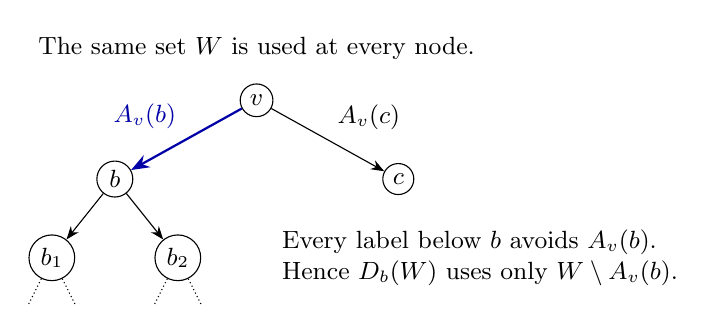
\begin{tikzpicture}[x=1cm,y=1cm,>=Stealth,
  vertex/.style={circle,draw,fill=white,inner sep=2pt},
  every node/.style={font=\small}]
\node[vertex] (v) at (0,0) {$v$};
\node[vertex] (b) at (-1.8,-1.0) {$b$};
\node[vertex] (c) at (1.8,-1.0) {$c$};
\node[vertex] (b1) at (-2.6,-2.0) {$b_1$};
\node[vertex] (b2) at (-1.0,-2.0) {$b_2$};
\draw[->,thick,blue!65!black] (v)--node[above left] {$A_v(b)$} (b);
\draw[->] (v)--node[above right] {$A_v(c)$} (c);
\draw[->] (b)--(b1);
\draw[->] (b)--(b2);
\draw[densely dotted] (b1)--(-2.9,-2.6);
\draw[densely dotted] (b1)--(-2.3,-2.6);
\draw[densely dotted] (b2)--(-1.3,-2.6);
\draw[densely dotted] (b2)--(-0.7,-2.6);
\node[align=left,anchor=west] at (0.2,-2.0)
  {Every label below $b$ avoids $A_v(b)$.\\
   Hence $D_b(W)$ uses only $W\setminus A_v(b)$.};
\node[anchor=south] at (0,0.4) {The same set $W$ is used at every node.};
\end{tikzpicture}
\caption{Every arc below $b$ lies on a path through the arc into $b$,
so $D_b$ is a function of coordinates outside the incoming label.
Labels on different branches (such as $A_v(c)$) may overlap $A_v(b)$.}
\label{fig:outside}
\end{figure}

\step{4}{one-level inequality}
Now let $W\sim\mu_\rho$. For a node $v$ with outgoing level $j$, take
expectations in \eqref{eq:pruning-recurrence}. Use \eqref{eq:Ed}. Use
\eqref{eq:Etf} with $f=D_b$, which is legitimate by Step~3 and
$D_b\ge0$. With $\epsilon_j^{-1}=\ee^{m_j}$ this gives
\begin{equation}\label{eq:expected-potential}
 \EE D_v(W)
 \le \ee^{m_j}\Bigl(\ee^{-9m_j}
    +\ee^{11m_j}\sum_{b\in\ch(v)}\nu_v(b)\,\EE D_b(W)\Bigr)
 = \ee^{-8m_j}
    +\ee^{12m_j}\sum_{b\in\ch(v)}\nu_v(b)\,\EE D_b(W).
\end{equation}

\step{5}{the root is bad with probability less than $\frac14$}
Define $\Phi_{k+1}=0$ and
$\Phi_j=\ee^{-8m_j}+\ee^{12m_j}\Phi_{j+1}$ for $j=k,k-1,\dots,1$.
\emph{Claim: $\EE D_v(W)\le\Phi_j$ for every node $v$ at depth $j-1$.}
Leaves are at depth $k$ and have $D=0=\Phi_{k+1}$. For a node at depth
$j-1\le k-1$ its children are at depth $j$. So
\eqref{eq:expected-potential}, the induction hypothesis and
$\sum_b\nu_v(b)=1$ give the claim. Unrolling the recursion,
\begin{equation}\label{eq:Phi}
 \Phi_1=\sum_{i=1}^{k}
 \exp\Bigl(12\,(m_1+\dots+m_{i-1})-8m_i\Bigr).
\end{equation}
Since $m_{i'}\le16^{-(i-i')}m_i$ for $i'<i$, we get
$m_1+\dots+m_{i-1}\le m_i\sum_{x\ge1}16^{-x}=m_i/15$. So the $i$-th
exponent is at most $(\tfrac{12}{15}-8)m_i\le-7m_i$. The $m_i$ are
strictly increasing positive integers, hence distinct. Therefore, for
the root $o$, by Step~2 and Markov's inequality,
\[
 \PP(o\text{ is bad})\le\PP(D_o(W)>1)\le\EE D_o(W)\le\Phi_1
 \le\sum_{m\ge1}\ee^{-7m}=\frac1{\ee^{7}-1}<\frac14 .
\]
So the procedure succeeds with probability at least $\frac34$.

\step{6}{the reduced tree}
Fix $W$ for which the root is good. Start from the root. At a good
non-leaf node $v$ with outgoing level $j$ put
\[
 \gamma_v(W)=\sum_{b\ \mathrm{good}}t_{vb}(W)\ge1-\epsilon_j>0 .
\]
Retain each good child $b$ with $t_{vb}(W)>0$. Give it weight
$t_{vb}(W)/\gamma_v(W)$. Replace its incoming label by
\[
 T_b=A_v(b)\setminus W,
\]
and continue recursively from $b$. Call the result $\TT'$. All
retained nodes are good. We verify the assertions.

\emph{(a) $\TT'$ is a probability tree with the same levels.} The
weights at a retained non-leaf node are positive and sum to
$\gamma_v/\gamma_v=1$. Since $\gamma_v>0$, at least one child is
retained. So every retained node at depth less than $k$ has a retained
child, and all leaves of $\TT'$ are at depth $k$.

\emph{(b) $\TT'$ is disjoint.} Every path of $\TT'$ is a path of
$\TT$, with each label replaced by a subset.

\emph{(c) Capacity.} If $b$ is retained then $t_{vb}(W)>0$. By
\eqref{eq:t-def} some pair $(c,b)$ has no local failure. In particular
$|T_b|=|A_v(b)\setminus W|\le m_j/2$, so
$|T_b|\le\lfloor m_j/2\rfloor$.

\emph{(d) Recovery \eqref{eq:recovery}.} Let $Q$ be a path of $\TT'$
and $P$ the same sequence of nodes viewed in $\TT$. On each arc,
$A_v(b)\subseteq W\cup T_b$. Taking unions gives
$\UU(P)\subseteq W\cup\UU(Q)$.

\emph{(e) Spread.} Let $v$ be a retained non-leaf node with outgoing
level $j$ and let $J\subseteq X$ be nonempty. Under the new child law
the probability that the label contains $J$ is
$\gamma_v(W)^{-1}\sum t_{vb}(W)$, summed over retained $b$ with
$J\subseteq T_b$. By \eqref{eq:t-def},
$t_{vb}(W)\le\sum_cK^v_W(c,b)$. If $K^v_W(c,b)>0$ and
$J\subseteq T_b$, then $J\subseteq T_b\subseteq A_v(c)$ by
Fact~A(a). Hence, using $\sum_bK^v_W(c,b)=\nu_v(c)$ from
\eqref{eq:kernel} and the $\alpha_j$-spread of $\nu_v$,
\[
 \sum_{b:\,J\subseteq T_b}t_{vb}(W)
 \le\sum_{c:\,J\subseteq A_v(c)}\ \sum_{b}K^v_W(c,b)
 =\sum_{c:\,J\subseteq A_v(c)}\nu_v(c)\le\alpha_j^{|J|}.
\]
In words, the fragment lies inside the \emph{source} label, and the
source has law $\nu_v$ at every fixed $W$. Dividing by
$\gamma_v\ge1-\epsilon_j$ and using $|J|\ge1$,
\[
 \PP_{\TT'}(J\subseteq\text{label at }v)
 \le\frac{\alpha_j^{|J|}}{1-\epsilon_j}
 \le\Bigl(\frac{\alpha_j}{1-\ee^{-m_j}}\Bigr)^{|J|}.
\]
Items (a)--(e) give (i) and (ii).
\end{proof}

\subsection{Iteration: proof of the tree theorem}\label{sec:iteration}

\begin{proof}[Proof of Theorem~\ref{thm:tree}]
\emph{Plan.} Apply Lemma~\ref{lem:reduction} repeatedly with fresh
random sets until every label is empty. Count how many sets are needed
and take their union.

\step{0}{parameters}
If $r=1$ then $W=X$ and the conclusion is trivial. Suppose $r<1$ and
set
\[
 a=4\sigma,\qquad \rho=\ee^{50}a=4\ee^{50}\sigma,
 \qquad s=\lfloor\log_2\ell_k\rfloor+1 .
\]
Since $1+\log_2\ell_k\ge1$, $r<1$ gives $16\ee^{50}\sigma<1$. So
$0<\rho<\frac14$. Also $2^{s-1}\le\ell_k<2^{s}$. For $\tau\ge0$ and
$1\le i\le k$ define
\begin{equation}\label{eq:capacities}
 m_i(\tau)=\left\lfloor\frac{\ell_i}{2^\tau}\right\rfloor,\qquad
 \alpha_i(\tau)=\sigma
 \prod_{\tau'=0}^{\tau-1}
 \left(1-\ee^{-m_i(\tau')}\right)^{-1}.
\end{equation}
Two facts about floors are used. For real $x\ge0$,
$\lfloor\lfloor x\rfloor/2\rfloor=\lfloor x/2\rfloor$. Indeed, if
$y=\lfloor x/2\rfloor$ then $2y\le x<2y+2$, so
$2y\le\lfloor x\rfloor<2y+2$. Hence
$\lfloor m_i(\tau)/2\rfloor=m_i(\tau+1)$. Also
$\lfloor16x\rfloor\ge16\lfloor x\rfloor$, so
$m_{i+1}(\tau)\ge\lfloor16\ell_i/2^\tau\rfloor\ge16\,m_i(\tau)$.

\step{1}{the procedure}
Let $W_1,W_2,\dots$ be independent sets of law $\mu_\rho$. Maintain a
current tree, initially $\TT_0=\TT$. Suppose $\tau<s$ successes have
occurred and the current tree is $\TT_\tau$. Attempt number $\lambda$
applies the procedure of Lemma~\ref{lem:reduction} to $\TT_\tau$ with
the set $W_\lambda$. A failed attempt leaves the tree unchanged. A
successful attempt returns a tree $\TT'$, which is trimmed as follows.
The levels $i$ of $\TT'$ with $m_i(\tau+1)=0$ form an initial segment,
since $m_i(\tau+1)$ is nondecreasing in $i$. By (i) all labels on them
are empty. By a fixed rule, follow one path from the root of $\TT'$
down through these levels to a node $w$. Let $\TT_{\tau+1}$ be the
subtree of $\TT'$ rooted at $w$. If no level remains, $\TT_{\tau+1}$
is a single node. Let $\lambda_\tau$ be the number of the $\tau$-th
successful attempt.

\step{2}{invariants}
\emph{Claim.} For $0\le\tau\le s$, once $\tau$ successes have
occurred:
\begin{enumerate}[label=(I\arabic*),leftmargin=2.8em,itemsep=2pt]
 \item $\TT_\tau$ is a disjoint probability tree whose levels are, in
 order, the original levels $i$ with $m_i(\tau)\ge1$. Level $i$ has
 capacity $m_i(\tau)$.
 \item Level $i$ of $\TT_\tau$ is $\alpha_i(\tau)$-spread, and
 $\alpha_i(\tau)\le4\sigma=a$.
 \item For every path $Q$ of $\TT_\tau$ there is a path $P$ of $\TT$
 with
 $\UU(P)\subseteq W_{\lambda_1}\cup\dots\cup W_{\lambda_\tau}\cup\UU(Q)$.
\end{enumerate}

\emph{The bound $\alpha_i(\tau)\le4\sigma$.} Let level $i$ be present
in $\TT_\tau$, so $m_i(\tau)\ge1$. The integers
$x_{\tau'}=m_i(\tau')$ satisfy
$x_{\tau'+1}=\lfloor x_{\tau'}/2\rfloor<x_{\tau'}$ whenever
$x_{\tau'}\ge1$. So $x_0>x_1>\dots>x_{\tau-1}\ge2$ are distinct
positive integers. The product in \eqref{eq:capacities} is thus at
most $\prod_{m\ge1}(1-\ee^{-m})^{-1}$. This is less than $4$. Using
$-\log(1-x)\le x/(1-x)\le x/(1-\ee^{-1})$ for $0\le x\le\ee^{-1}$,
\begin{equation}\label{eq:product}
 \sum_{m=1}^{\infty}-\log(1-\ee^{-m})
 \le \frac{1}{1-\ee^{-1}}\sum_{m=1}^{\infty}\ee^{-m}
 =\frac{\ee^{-1}}{(1-\ee^{-1})^2}<0.93<\log 4 .
\end{equation}

\emph{Induction.} For $\tau=0$, (I1)--(I3) are the hypotheses (with
$P=Q$). Assume them for some $\tau<s$. By (I1), (I2) and Step~0,
$\TT_\tau$ satisfies the hypotheses of Lemma~\ref{lem:reduction}. The
capacities $m_i(\tau)$ are positive integers with
$m_{i+1}(\tau)\ge16m_i(\tau)$. The spread parameters satisfy
$\alpha_i(\tau)\le a$. And $\rho=\ee^{50}a<1$. $\TT_\tau$ has at least
one level because $m_k(\tau)\ge1$ for $\tau\le s-1$. On success the
lemma returns a disjoint tree $\TT'$ whose level $i$ has capacity
$\lfloor m_i(\tau)/2\rfloor=m_i(\tau+1)$ and is
$\alpha_i(\tau)/(1-\ee^{-m_i(\tau)})=\alpha_i(\tau+1)$-spread.
Trimming preserves these. A subtree of a disjoint probability tree is
one, capacity and spread are conditions on single nodes, and exactly
the levels with $m_i(\tau+1)\ge1$ remain. This gives (I1) and (I2)
for $\tau+1$. For (I3), let $Q'$ be a path of $\TT_{\tau+1}$.
Prefixing the trimmed path from the root of $\TT'$ to $w$, whose
labels are empty, gives a path $Q$ of $\TT'$ with $\UU(Q)=\UU(Q')$.
By \eqref{eq:recovery} there is a path $P'$ of $\TT_\tau$ with
$\UU(P')\subseteq W_{\lambda_{\tau+1}}\cup\UU(Q')$. By (I3) for
$\tau$ there is a path $P$ of $\TT$ with
$\UU(P)\subseteq W_{\lambda_1}\cup\dots\cup W_{\lambda_\tau}\cup\UU(P')$.
Combine the two inclusions.

\step{3}{after $s$ successes a path is covered}
Since $\ell_i\le\ell_k<2^s$, $m_i(s)=0$ for all $i$. By (I1), $\TT_s$
is a single node. Its only path $Q$ has $\UU(Q)=\varnothing$. By (I3)
there is a path $P$ of $\TT$ with
\[
 \UU(P)\subseteq W_{\lambda_1}\cup\dots\cup W_{\lambda_s}.
\]

\step{4}{$4s$ attempts suffice with probability $\frac23$}
Before attempt $\lambda$ the current tree is a function of
$W_1,\dots,W_{\lambda-1}$. Conditionally on these, $W_\lambda$ still
has law $\mu_\rho$. So by Lemma~\ref{lem:reduction} and Step~2 the
attempt succeeds with conditional probability at least $\frac34$. Let
$\xi_\tau=\lambda_\tau-\lambda_{\tau-1}$ (with $\lambda_0=0$) be the
number of attempts used for the $\tau$-th success. Decomposing
according to the value of $\lambda_{\tau-1}$ and conditioning on the
draws so far gives
$\PP(\xi_\tau>x+1)\le\frac14\PP(\xi_\tau>x)$. Hence
$\PP(\xi_\tau>x)\le4^{-x}$ and
$\EE\xi_\tau=\sum_{x\ge0}\PP(\xi_\tau>x)\le\frac43$. Thus
$\EE\lambda_s\le\frac43s$, and by Markov's inequality
\[
 \PP(\lambda_s>4s)\le\frac{\EE\lambda_s}{4s}\le\frac13 .
\]

\step{5}{conclusion}
Let $W_*=W_1\cup\dots\cup W_{4s}$. On the event $\lambda_s\le4s$,
which has probability at least $\frac23$, Step~3 gives a path $P$ with
$\UU(P)\subseteq W_*$. By (P3) and Bernoulli's inequality, $W_*$ has
law $\mu_{r_*}$ with
\[
 r_*=1-(1-\rho)^{4s}
 \le4s\rho
 =16\ee^{50}\sigma s
 \le16\ee^{50}\sigma(1+\log_2\ell_k)=r .
\]
The event ``$\UU(P)\subseteq W$ for some path $P$'' is closed under
enlarging $W$. By (P2) its probability under $\mu_r$ is at least that
under $\mu_{r_*}$, hence at least $\frac23$.
\end{proof}

\emph{Sanity check.} For $k=1$ the tree is a single $\sigma$-spread
family of sets of size at most $\ell_1$. The theorem then says that a
random set of density $O(\sigma\log(2\ell_1))$ contains a member with
probability at least $\frac23$.

\section{Application to graph containment}\label{sec:graphs}

It remains to build, for the given $H$, a tree satisfying the
hypotheses of Theorem~\ref{thm:tree}.

\subsection{Conventions for copies}

Put $q=\pE(n,H)$ and $\sigma=128q$. By facts (b) and (c) of
Section~\ref{sec:introduction}, $q>0$ and every constraint in the
definition of $\pE$ holds at $p=q$.

\emph{Isolated vertices.} Delete the isolated vertices of $H$. This
does not change the event of containing $H$. A copy of the remaining
graph in a graph on $[n]$ extends to a copy of the original $H$ by
assigning the deleted vertices to unused vertices of $[n]$. This is
possible since $H$ had at most $n$ vertices and copies need not be
induced. The number $q$ remains the threshold of the \emph{original}
$H$.

\emph{Edge sets.} From now on a graph without isolated vertices is
identified with its edge set, and $H$ also denotes its own edge set, so
$|H|=h$. An edge set $F$ has vertex set $V(F)$, the set of endpoints of
its edges. Two edge sets are isomorphic if a bijection of vertex sets
carries one onto the other. Let $X=\binom{[n]}2$. A \emph{copy of $F$
on $[n]$} is a subset of $X$ isomorphic to $F$. For edge sets $F$ and
$I$ let
\[
 M(F)=\#\{\text{copies of $F$ on $[n]$}\}=N(K_n,F),\qquad
 M(I,F)=\#\{F'\subseteq I:\ F'\cong F\}=N(I,F).
\]
A subgraph isomorphic to a graph without isolated vertices is
determined by its edge set, so these are the ordinary copy counts. (In
terms of vertex maps, $M(F)=(n)_{v(F)}/|\operatorname{Aut}(F)|$ with
$(n)_v=n(n-1)\cdots(n-v+1)$. This formula is not needed.) Set
$M(\varnothing)=M(I,\varnothing)=1$. Every edge subset $F\subseteq H$,
on its vertex set, is a subgraph of the original $H$ and has at most
$n$ vertices.

\begin{fact}[Copy ratio]\label{fact:C}
Let $F\subseteq I$ be edge sets with $|V(I)|\le n$. Let
$\boldsymbol I$ be a uniformly random copy of $I$ on $[n]$ and $F_0$
any fixed copy of $F$ on $[n]$. Then
\begin{equation}\label{eq:copy-ratio}
 \PP(F_0\subseteq\boldsymbol I)=\frac{M(I,F)}{M(F)}.
\end{equation}
\end{fact}

\begin{proof}
A permutation of $[n]$ maps the set of copies of $I$ bijectively to
itself, so it preserves the law of $\boldsymbol I$. Any copy of $F$
can be mapped to any other by a permutation of $[n]$. Hence
$\PP(F_0\subseteq\boldsymbol I)$ is the same for all $M(F)$ copies
$F_0$. Summing over them gives the expected number of copies of $F$
contained in $\boldsymbol I$. This number is $M(I,F)$, because
$\boldsymbol I\cong I$.
\end{proof}

\begin{fact}[First moments at $q$]\label{fact:D}
For every nonempty edge subset $F\subseteq H$,
\begin{equation}\label{eq:fm}
 M(F)\,q^{|F|}\ge\tfrac12 .
\end{equation}
\end{fact}

\begin{proof}
$F$ is a subgraph of the original $H$. So its constraint
$\EE N(G(n,q),F)\ge\frac12$ holds at $q=\pE(n,H)$. By
\eqref{eq:firstmoment} the left side is $M(F)q^{|F|}$.
\end{proof}

\subsection{The hierarchy}

\begin{lemma}[Graph hierarchy]\label{lem:hierarchy}
There is a disjoint probability tree on
$X=\binom{[n]}2$ whose path unions are copies of $H$ with its isolated
vertices removed, such that every level is $\sigma$-spread and its label
sizes $\ell_1,\ldots,\ell_k$ satisfy
\[
 1\le\ell_1,\qquad \ell_{i+1}\ge16\ell_i,
 \qquad \ell_k\le e(H).
\]
\end{lemma}

Here $\sigma=128q$, all labels on level $i$ have size exactly
$\ell_i$, and $k\ge1$. The lemma is used once, in the proof of
Theorem~\ref{thm:main}.

\begin{proof}
\emph{Plan.} Peel $H$ down to $\varnothing$ by repeatedly passing to a
subset that maximises a normalised containment probability. Fact~D
makes each step shrink the edge set by a factor of more than $17$.
Maximality is exactly the spread condition for the extension back up.

\step{1}{a maximiser is small}
For a nonempty edge set $I\subseteq H$ and $S\subseteq I$ define
\begin{equation}\label{eq:maximizer}
 R_\sigma(I,S)=\sigma^{-|S|}\,\PP(S_0\subseteq\boldsymbol I),
\end{equation}
where $\boldsymbol I$ is a uniform copy of $I$ on $[n]$ and $S_0$ is
any fixed copy of $S$. By Fact~C this does not depend on $S_0$. Note
$R_\sigma(I,\varnothing)=1$. Let $S\ne\varnothing$. By
\eqref{eq:copy-ratio}, \eqref{eq:fm} for $F=S$, and
$M(I,S)\le\binom{|I|}{|S|}$ (copies of $S$ in $I$ are $|S|$-element
subsets of $I$),
\[
 R_\sigma(I,S)=\sigma^{-|S|}\frac{M(I,S)}{M(S)}
 \le\sigma^{-|S|}\binom{|I|}{|S|}\,2q^{|S|}
 =2\binom{|I|}{|S|}128^{-|S|}.
\]
If moreover $|S|\ge|I|/17$, then
$\binom{|I|}{|S|}\le(\ee|I|/|S|)^{|S|}\le(17\ee)^{|S|}$ gives
\begin{equation}\label{eq:small}
 R_\sigma(I,S)\le2\left(\frac{17\ee}{128}\right)^{|S|}<1 ,
\end{equation}
because $17\ee/128<0.37$ and $|S|\ge1$. Since the empty set has value
$1$, every maximiser $S$ of $R_\sigma(I,\cdot)$ over subsets of $I$
satisfies $|S|<|I|/17$. In particular $S\ne I$.

\step{2}{the chain}
Start with $I=H$. Choose a maximiser $S$ of $R_\sigma(I,\cdot)$ by a
fixed tie-breaking rule. Replace $I$ by $S$ and repeat until
$S=\varnothing$. Sizes strictly decrease, so this terminates. In
reverse order the sets form a chain
\[
 \varnothing=H_0\subset H_1\subset\cdots\subset H_k=H,
 \qquad |H_{i-1}|<|H_i|/17,\qquad k\ge1,
\]
in which $H_{i-1}$ maximises $R_\sigma(H_i,\cdot)$ over all edge
subsets of $H_i$.

\step{3}{the tree}
The root is $\varnothing$, the unique copy of $H_0$. A node at depth
$i-1$ is a copy $S_0$ of $H_{i-1}$ on $[n]$ together with its history.
Distinct histories are distinct nodes. Its children are all copies
$I_0$ of $H_i$ on $[n]$ with $I_0\supseteq S_0$, with the uniform
distribution. The arc to $I_0$ has label $I_0\setminus S_0$. Children
exist. Indeed, $S_0$ is the image of $H_{i-1}$ under an injection
$V(H_{i-1})\to[n]$. This extends to an injection $V(H_i)\to[n]$
because $|V(H_i)|\le n$, and the image of $H_i$ is a copy containing
$S_0$. So this is a probability tree with $k$ levels.

\step{4}{disjointness and sizes}
Along a path the copies are nested,
$\varnothing\subset I_1\subset\dots\subset I_k$, and the labels are
the successive differences. They are pairwise disjoint with union
$I_k$, a copy of $H$. Every label on level $i$ has size
$\ell_i=|H_i|-|H_{i-1}|\ge1$. Moreover
\[
 \ell_{i+1}=|H_{i+1}|-|H_i|>17|H_i|-|H_i|=16|H_i|\ge16\ell_i,
 \qquad \ell_k\le|H_k|=e(H).
\]

\step{5}{spread}
Fix a node $S_0$ at depth $i-1$ and a nonempty $J\subseteq X$. Let $A$
be the random label of the arc to its child. The child is uniform
among the copies of $H_i$ containing $S_0$. That is, it has the law of
a uniform copy $\boldsymbol I$ of $H_i$ conditioned on
$S_0\subseteq\boldsymbol I$, and $A=\boldsymbol I\setminus S_0$. If
$J\cap S_0\ne\varnothing$ then $\PP(J\subseteq A)=0$. Otherwise
\begin{equation}\label{eq:conditional-ratio}
 \PP(J\subseteq A)=
 \frac{\PP(S_0\cup J\subseteq\boldsymbol I)}
      {\PP(S_0\subseteq\boldsymbol I)} .
\end{equation}
If the numerator is zero there is nothing to prove. If it is positive,
$S_0\cup J$ lies in some copy of $H_i$. Pulling back along the
isomorphism, $S_0\cup J$ is a copy of an edge subset $U\subseteq H_i$
with $|U|=|S_0|+|J|$. Also $S_0$ is a copy of $H_{i-1}$. Maximality of
$H_{i-1}$ gives $R_\sigma(H_i,U)\le R_\sigma(H_i,H_{i-1})$, that is,
\[
 \sigma^{-(|S_0|+|J|)}\,\PP(S_0\cup J\subseteq\boldsymbol I)
 \le \sigma^{-|S_0|}\,\PP(S_0\subseteq\boldsymbol I).
\]
With \eqref{eq:conditional-ratio} this is
$\PP(J\subseteq A)\le\sigma^{|J|}$. So every level is $\sigma$-spread.
\end{proof}

\emph{Sanity check.} If $H$ is a single edge then $q=1/(2\binom n2)$,
$k=1$, and the root's children are the $\binom n2$ edges with uniform
weights. Spread requires $1/\binom n2\le128q$, and indeed
$1/\binom n2=2q$.

\subsection{Proof of the main theorem}

\begin{proof}[Proof of Theorem~\ref{thm:main}]
The tree of Lemma~\ref{lem:hierarchy} is a disjoint probability tree
on $X=\binom{[n]}2$ with $k\ge1$ levels. Every level is
$\sigma$-spread with $\sigma=128q>0$. Level $i$ has capacity $\ell_i$,
a positive integer, and $\ell_{i+1}\ge16\ell_i$.
Theorem~\ref{thm:tree} applies. So a random edge set of density
$\min\{1,16\ee^{50}\cdot128q\,(1+\log_2\ell_k)\}$ contains $\UU(P)$
for some path $P$ with probability at least $\frac23$. This $\UU(P)$
is a copy of $H$ without its isolated vertices. Since $\ell_k\le h$
and $16\cdot128=2048$, this density is at most
\[
 r=\min\{1,\;2048\ee^{50}q(1+\log_2 h)\}.
\]
By (P2) the same holds at density $r$. A random edge set of density
$r$ on $X$ is $G(n,r)$. By the remark on isolated vertices, $G(n,r)$
contains a copy of the original $H$ with probability at least
$\frac23\ge\frac12$. Hence $\pc(n,H)\le r$, which is
\eqref{eq:stronger}.

Finally, $h\le\binom n2\le n^2$ and $\log_2n\ge1$ give
$1+\log_2h\le1+2\log_2n\le3\log_2n$. So
$\pc(n,H)\le3\cdot2048\,\ee^{50}q\log_2n=6144\,\ee^{50}\pE(n,H)\log_2n$.
\end{proof}

\section{Verification checklist}\label{sec:checklist}

These are the steps on which the argument rests, in suggested order of
checking.

\begin{enumerate}[leftmargin=2em,itemsep=4pt]
 \item \textbf{Locality of the potential} (Lemma~\ref{lem:reduction},
 Step~3). $D_b(W)$ must be a function of $W$ outside the incoming
 label $A_v(b)$. This is the only place where disjointness along paths
 is used for the probability estimate. Check that $d_u$ and $t_{uc}$
 are defined from the \emph{fixed input tree} for all nodes, not from
 the pruned tree, and that they inspect $W$ only on the child labels
 of $u$ (Fact~A(b)).
 \item \textbf{Distortion bound} \eqref{eq:distortion}
 (Lemma~\ref{lem:local}, Steps~2 and~6). The independence in
 \eqref{eq:master-f} needs $f$ to depend only on $W\setminus A_b$ and
 the indicator only on $W\cap A_b$. The exponent bookkeeping is
 $\rho^{-|A_b|}\rho^{|A_b\setminus A_c|}=\rho^{-|A_c\cap A_b|}$.
 \item \textbf{Exponent arithmetic in the potential}
 (Lemma~\ref{lem:reduction}, Steps~4--5).
 $\ee^{m}\ee^{-9m}=\ee^{-8m}$ and $\ee^{m}\ee^{11m}=\ee^{12m}$. Then
 $12\cdot\frac1{15}-8\le-7$ uses $m_{j+1}\ge16m_j$, and distinctness
 of the $m_j$ gives the bound $\sum_{m\ge1}\ee^{-7m}<\frac14$.
 \item \textbf{Failure bound} \eqref{eq:local-failure}
 (Lemma~\ref{lem:local}, Steps~1, 4, 5). The density identity of
 Fact~B, the implication
 $|T|>m/2\Rightarrow|A_c\cap A_b|>m/2$ from Fact~A(a), and
 $\ee^{-10m}+2^m\ee^{-15m}\le\ee^{-9m}$.
 \item \textbf{Spread of the reduced tree}
 (Lemma~\ref{lem:reduction}, Step~6(e)). The fragment is compared with
 the source, whose law is $\nu_v$ at every fixed $W$. The only loss is
 the normalisation $\gamma_v\ge1-\ee^{-m_j}$, which needs the retained
 node to be good.
 \item \textbf{Accumulated spread loss and attempt count}
 (Theorem~\ref{thm:tree}, Steps~2 and~4). The capacities
 $\lfloor\ell_i/2^{\tau'}\rfloor$ entering the product are distinct
 positive integers and $\prod_{m\ge1}(1-\ee^{-m})^{-1}<4$
 \eqref{eq:product}. Each attempt uses a fresh set, so the $\frac34$
 bound holds conditionally on the past.
 \item \textbf{The hierarchy} (Lemma~\ref{lem:hierarchy}, Steps~1
 and~5). Fact~D is applied to $S$ as a subgraph of the original $H$
 with ordinary copy counts. $2(17\ee/128)^{|S|}<1$ forces
 $|S|<|I|/17$. Maximality is over \emph{all} edge subsets of $H_i$, so
 it covers the set $U\cong S_0\cup J$.
 \item \textbf{Constants} (proofs of Theorems~\ref{thm:tree}
 and~\ref{thm:main}). $\rho=4\ee^{50}\sigma$, $4s$ draws with
 $s\le1+\log_2\ell_k$, and $\sigma=128q$, giving
 $4\cdot4\cdot128=2048$ and $3\cdot2048=6144$.
\end{enumerate}

\begin{thebibliography}{99}
\raggedright

\bibitem{ALWZ21}
R.~Alweiss, S.~Lovett, K.~Wu, and J.~Zhang,
\emph{Improved bounds for the sunflower lemma},
Annals of Mathematics (2) \textbf{194} (2021), no.~3, 795--815.
\href{https://doi.org/10.4007/annals.2021.194.3.5}{doi:10.4007/annals.2021.194.3.5}.

\bibitem{Bollobas81}
B.~Bollob\'as,
\emph{Threshold functions for small subgraphs},
Mathematical Proceedings of the Cambridge Philosophical Society
\textbf{90} (1981), no.~2, 197--206.
\href{https://doi.org/10.1017/S0305004100058655}{doi:10.1017/S0305004100058655}.

\bibitem{DKP25}
Q.~Dubroff, J.~Kahn, and J.~Park,
\emph{On the ``second'' Kahn--Kalai conjecture},
arXiv:2508.14269v1 (August 19, 2025).
\url{https://arxiv.org/abs/2508.14269v1}.

\bibitem{DKP25Cases}
Q.~Dubroff, J.~Kahn, and J.~Park,
\emph{On the ``second'' Kahn--Kalai conjecture: cliques, cycles, and trees},
arXiv:2510.02005v2 (October 23, 2025).
\url{https://arxiv.org/abs/2510.02005v2}.

\bibitem{ER60}
P.~Erd\H{o}s and A.~R\'enyi,
\emph{On the evolution of random graphs},
Publications of the Mathematical Institute of the Hungarian Academy of
Sciences \textbf{5} (1960), 17--61.
\url{https://static.renyi.hu/~p_erdos/1960-10.pdf}.

\bibitem{ER66}
P.~Erd\H{o}s and A.~R\'enyi,
\emph{On the existence of a factor of degree one of a connected random graph},
Acta Mathematica Academiae Scientiarum Hungaricae
\textbf{17} (1966), 359--368.
\url{https://users.renyi.hu/~p_erdos/1966-16.pdf}.

\bibitem{FKNP21}
K.~Frankston, J.~Kahn, B.~Narayanan, and J.~Park,
\emph{Thresholds versus fractional expectation-thresholds},
Annals of Mathematics (2) \textbf{194} (2021), no.~2, 475--495.
\href{https://doi.org/10.4007/annals.2021.194.2.2}{doi:10.4007/annals.2021.194.2.2}.

\bibitem{KK07}
J.~Kahn and G.~Kalai,
\emph{Thresholds and expectation thresholds},
Combinatorics, Probability and Computing
\textbf{16} (2007), no.~3, 495--502.
\href{https://doi.org/10.1017/S0963548307008474}{doi:10.1017/S0963548307008474}.

\bibitem{LSZ19}
S.~Lovett, N.~Solomon, and J.~Zhang,
\emph{From DNF compression to sunflower theorems via regularity},
34th Computational Complexity Conference, LIPIcs \textbf{137} (2019),
5:1--5:14.
\href{https://doi.org/10.4230/LIPIcs.CCC.2019.5}{doi:10.4230/LIPIcs.CCC.2019.5}.

\bibitem{MNSZ25}
E.~Mossel, J.~Niles-Weed, N.~Sun, and I.~Zadik,
\emph{A Bayesian proof of the spread lemma},
Random Structures \& Algorithms \textbf{66} (2025), no.~4, e70008.
\href{https://doi.org/10.1002/rsa.70008}{doi:10.1002/rsa.70008}.

\bibitem{MNSZ22}
E.~Mossel, J.~Niles-Weed, N.~Sun, and I.~Zadik,
\emph{On the second Kahn--Kalai conjecture},
arXiv:2209.03326v1 (September 7, 2022).
\url{https://arxiv.org/abs/2209.03326v1}.

\bibitem{OpenAIThresholdEquivalence2026}
OpenAI,
\emph{Integral and fractional expectation thresholds are equivalent},
OpenAI Math Release preprint
\href{https://github.com/openai/math/blob/main/preprints/Integral-and-fractional-expectation-thresholds-are-equivalent-September-23-2026/paper.pdf}{OAI:Integral-and-fractional-expectation-thresholds-are-equivalent-September-23-2026},
2026, Theorem~1.1, p.~2.

\bibitem{PP24}
J.~Park and H.~T.~Pham,
\emph{A proof of the Kahn--Kalai conjecture},
Journal of the American Mathematical Society
\textbf{37} (2024), no.~1, 235--243.
\href{https://doi.org/10.1090/jams/1028}{doi:10.1090/jams/1028}.

\bibitem{Riordan00}
O.~Riordan,
\emph{Spanning subgraphs of random graphs},
Combinatorics, Probability and Computing
\textbf{9} (2000), no.~2, 125--148.
\href{https://doi.org/10.1017/S0963548399004150}{doi:10.1017/S0963548399004150}.

\bibitem{Tal10}
M.~Talagrand,
\emph{Are many small sets explicitly small?},
Proceedings of the 42nd ACM Symposium on Theory of Computing (2010),
13--36.
\href{https://doi.org/10.1145/1806689.1806693}{doi:10.1145/1806689.1806693}.

\bibitem{Tran26}
T.~Tran,
\emph{Fractional expectation thresholds and the ``second'' Kahn--Kalai
conjecture},
arXiv:2609.20546v2 (September 24, 2026).
\url{https://arxiv.org/abs/2609.20546v2}.

\end{thebibliography}

\end{document}
